%      Awab you idiot. WHy you do this
%      ps. hi person reading this (probs sukaina)

\documentclass{article}
\usepackage[utf8]{inputenc}
\usepackage[T1]{fontenc}
\usepackage{microtype}
\usepackage{graphicx}
\setlength{\parindent}{2pt}
%To get rid of indents cause miss amna hates them 
\usepackage{fancyhdr}
\usepackage{float}
\usepackage{lipsum}
\usepackage{newspaper}
%that's the one which makes the magic happen
\usepackage{newspaper-mod}
%%to redefine the headline and byline style if you want to.
%% These can be issued just before any
%% byline or headline in the paper, to
%% individually style each article
%%
% \renewcommand{\headlinestyle}{\itshape\Large\lsstyle}
% \renewcommand{\bylinestyle}{\bfseries\Large\raggedright}

\usepackage{multicol}
%For making columns using command \begin{multicols}{2}....\end{multicols}

%Fancy images
\usepackage{picinpar}
%uasage of picinpar:
%\begin{window}[1,l,\includegraphics{},caption]xxxxx\end{window}

% \begin{window}[2,r,\includegraphics[width=1.0in]{atom.jpg},\centerline{The Atom}] The \verb+multicol+ package allows using multiple columns without starting a new page.  Using floats is not possible in a columns environment, however with the \verb+picinpar+ package, I can set a picture inside a block of text---just like you one you see here.  Isn't \LaTeX{} cool?
% And now we're just filling more space, and yet more space.  
% \end{window}


% TODO: Change the font to Times New Roman



%Metadata you shouldn't change
\SetPaperName{
          %  
\includegraphics[scale=0.3]{fps}
        % \scalerel*{
\includegraphics{fps}}{f}
            FPS Eagles:   
         \hfill  
\includegraphics[height=\fontcharht\font`\B]{cfps} 
      }
\SetHeaderName{FPS Eagles}
\SetPaperLocation{
%    \centering
   %\begin{figure}
    %   \centering
  %  \vspace{5mm}
  %  
\includegraphics[scale=0.12]{lfps} 
   %  
\includegraphics[scale=0.09]{W}
   %\end{figure}
    
   
}
\SetPaperSlogan{
            %     
\includegraphics[scale=0.3]{fps}
                ``\textit{FPSonians are the best; second to none!}''
              %  
\includegraphics[scale=0.1]{cfps}
                }
\SetPaperPrice{By Awab Qureshi and Sukaina Kazmi; batch 2020}
\cfoot{\textit{FPSonians are the best; second to none!}}


% Metadata you should change
\date{\today}
\currentvolume{1}
\currentissue{1}




\begin{document}
\maketitle
\large 

%The beginning 

%                               FRONT PAGE

\headline{main}\textbf{by}

\closearticle
%do \closearticle for that double line bar

\begin{multicols}{2}
%to make columns

\headline{side 1}\textbf{by}




\headline{side 2}\textbf{by}


\end{multicols}
\pagebreak 
%to make sure stuff stays on this page


%                               2ND PAGE

\headline{current affair editorial}\textbf{by }

\closearticle

\begin{multicols}{2}
\headline{Sports}

\closearticle


\headline{This Week in History}

\closearticle

\headline{Upcoming Events}

\closearticle
\end{multicols}

\pagebreak

%                              3RD PAGE 

\headline{What's Up With Tech?}
\begin{multicols}{2}
    \headline{tech 1}

%\closearticle


\headline{tech 2}

%\vfill
%\closearticle

\end{multicols}
\closearticle

\begin{center}
\headline{Jokes, and Memes}
%
\includegraphics{m1.jpeg}
%
\includegraphics{m2.jpeg}
%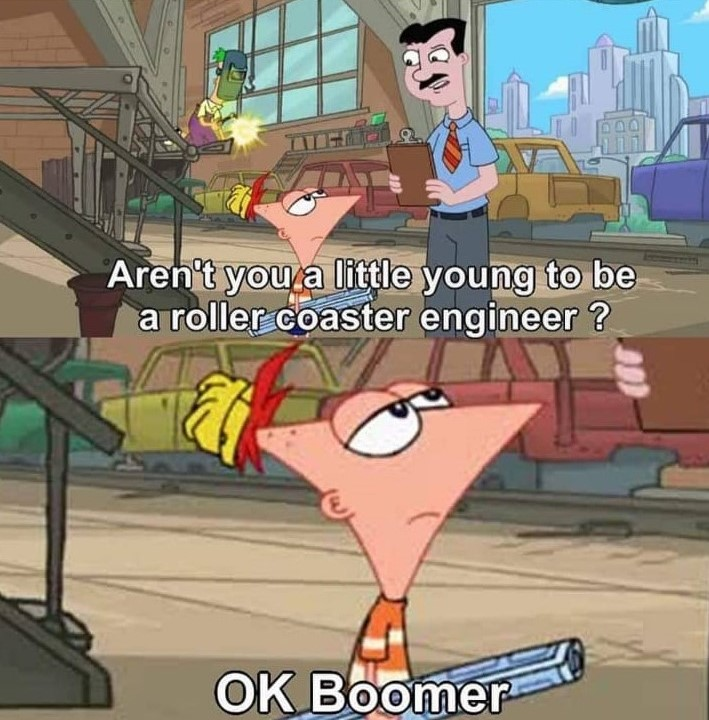
\includegraphics{m3.jpeg}
%
\includegraphics{m4.jpeg}
\end{center}

\pagebreak


%                            4TH PAGE

\begin{multicols}{2}

\headline{world 1}

\pagebreak


\end{multicols}

\end{document}
